% SOS Spectrometer information

\section{Short Orbit Spectrometer (SOS) }

The SOS is composed of one quadrupole and two dipole magnets.
These are all conventional resistive magnets and are powered by standard
power supplies.
The first dipole deflects particles by 33 degrees, while the
second dipole deflects by 15 degrees in the opposite direction, such
that the total bend of the SOS dipoles is 18 degrees.
The two dipole magnets are enclosed in a common yoke.

The SOS quadrupole was assembled at Argonne National Laboratory and
subsequently shipped to JLab. The dipole is a copy of the Medium Resolution
Spectrometer of Los Alamos, and has been assembled at JLab by a collaboration
of Argonne National Laboratory, Los Alamos, and JLab.

The magnet system is followed by a large concrete detector (or shielding) hut,
in which all detector elements can be found. All of these
detector elements have been built by universities and laboratories involved 
in the Hall~C
physics program.

The SOS magnet system combines a large acceptance (solid angle and momentum
acceptance) with a relatively short path length to the focal plane.
The primary object of this spectrometer is to detect short-lived particles
like pions and kaons. In addition, a large fraction of the experimental
program in Hall~C requires a spectrometer with large momentum and solid angle
acceptance to maximize the operational efficiency.
The maximum central momentum attainable with the SOS magnet system is 1.8 GeV/c.

\section{SOS Magnets and Power Supplies }

The SOS magnets are powered by large supplies
(160 Volt, 1000 Amps for Quad and D2, 250 Volts, 1000 Amps for D1).
When working on the power supplies, the responsible people will follow
the guidelines in the electrical safety chapter of the `` JLab EH$\&$S
Manual." Further references which should be consulted before power supply
maintenance or operations are attempted are the operating procedure
provided by the manufacture (Inverpower) and the simplified magnet
power supply maintenance procedure.
The connections at the quadrupole are covered with a 1/4 plexiglass, so that they are not exposed.
The cabinet doors for the power supplies are locked.
There is also a crash button in the counting house which is interlocked with
a separate key. When the key is locked off, in crash mode, the power supply
cannot be energized.
In case you need any of the keys, see the Responsible Personnel listed in 
the \htmladdnormallinkfoot{ESAD}{http://www.jlab.org/Hall-C/document}.

Signs have been posted which indicate the presence of a high magnetic
field ( these are standard JLab safety signage). The exact wording is
``High Magnetic Field - No Pacemakers or Credit Cards." There
are also flashing red lights located near the exit of the last dipole
and near the entrance of the dipole at the pivot that indicate that the
magnet power supplies are energized.

The magnets and their power supplies
are cooled by the Hall~C Low Conductivity Water system (LCW).
The LCW system for the dipole and quadrupoles has been
plumbed using hoses rated for 600 PSI. These hoses have been tested during
the magnet mapping. The cooling water is delivered at 240 PSI.

The spectrometer is in Hall~C and the power supplies are located
behind the blue electronics racks on the HMS side of the hall.
The control of the magnets is available through VME, and will be
described in a subsequent Section.


\subsection{SOS Magnet - Description}

The SOS consists of 3 magnets: a quadrupole (QS), followed by two dipoles housed
in a common yoke (BM01 and BM02). All three are resistive magnets
with pressurized water cooling. They are powered by 3
InverPower remotely controlled power supplies, located in the blue racks at
the north side of Hall~C. Group-3 Digital Tesla meter hall probes
are used to monitor the magnetic fields.

The magnets are aligned as a vertical-bend Q, D, -D spectrometer: BM01 bends
charge=1 particles of the central momentum upwards by 33 degrees, and BM02 bends
the central ray down by 15 degrees, resulting in a slope of 18 degrees through
the detectors. QS focuses in the non-bend plane, and defocuses in the bend
plane. Focusing in the bend plane is provided by the dipoles, which have tilted
and curved entrance and exit edges. The ``standard" tune has first-order
point-to-point focusing in both the bend and non-bend planes at the ``standard"
reconstruction plane, located approximately at the first drift chamber (DC1).
An alternate tune with parallel-to-point focusing in the non-bend plane can be
achieved by lowering the excitation of QS and changing the location of the
focal plane. The power-supplies contain a motorized internal bus that can 
reverse
the output polarity so that operation for either positive or negatively charged
particles is possible.

Both BM01 and BM02 require an asymptotic field (far from the edges) of 11379.3
Gauss/GeV for the central ray. While the center of BM01 is far from the edges,
BM02 is a thin magnet, and there is no region that isn't close to the entrance
and exit edges. The proper relative excitation of these magnets is determined
by numerically integrating the central ray's trajectory through the fields
measured during the mapping of these magnets, and by comparing the observed and
expected trajectories of the central ray through the drift chambers.

The ``standard tune" requires a gradient of approximately 498.152 Gauss/cm/GeV
in QS. The excitation of QS relative to BM01 was determined by observing
electrons that passed through a sieve-slit mask at the entrance to QS after
scattering elastically from a carbon target. The field in QS was varied until
the correct focus was observed at the reconstruction plane.

The maximum central momentum of the spectrometer is approximately 1.75 GeV.
This limit is imposed by the power supplies; at this setting BM01 requires
approximately 1000 amps, and QS requires approximately 170 volts. 
Table~\ref{tab:sos_ratings}
lists the maximum output voltage and current of each power supply. However, the
iron in the magnets is significantly saturated at this setting, and a 
significant
increase in the central momentum probably can't be achieved without affecting
the optics.

\begin{table}
\begin{center}
\caption{Maximum ratings of SOS power supplies. \label{tab:sos_ratings}}
\vspace{\baselineskip}
  \begin{tabular}{lll}
Magnet         &Max Current    &Max Voltage    \\
                     &~~~~~(A)        &~~~~~(V)              \\
\hline
BM01           &1000 (*)       &250            \\
BM02           &1000           &160            \\
QUAD           &1000           &160 (**)       \\
\end{tabular}
\end{center}
\noindent{(*)  Limits max momentum setting of spectrometer}\newline
\noindent{(**) The quad is driven to $\approx$170 volts at 1.75 GeV, but this
is within the overdrive capability of the supply.}

\end{table}

All three magnets are equipped with Group-3 precision hall-effect probes to
monitor their fields. BM01 and BM02 are equipped with LPT-141 probes that are
glued onto the pole tips inside the magnet vacuum with Torr seal epoxy. The cables
from the probes are routed inside the magnets to the transition vacuum piece
between QS and BM01, where they pass through a feed-through. The BM01 probe was
placed near the center of the pole, in the uniform field region. The BM02 probe
was placed near the widest part of the pole. in both cases, the probe location
is outside of the beam envelope accepted by the spectrometer.

QS is equipped with a LPT-130 probe located in an aluminum holder mounted in an
access hole of one of the stainless-steel spacers between the upper and lower
pole pieces. This positions the probe in the horizontal midplane of the magnet,
in the region where the upper and lower pole pieces are closest together. The
field at this point is proportional to the field gradient in the magnet bore, in
the absence of saturation. Saturation effects are estimated by the 2D magnet
code Poisson, but the precise tune of the magnet relative to BM01 can only be
determined experimentally.

The cables for all three hall-probes are bundled together at the transition
piece between QS and BM01. The cables for BM01 and BM02 have a connector that
attaches to the feed thrus on the top of the transition piece. (There is a
corresponding connector inside the magnet vacuum.) The feed thru for BM01 is
the one closest to the target. It is extremely important that the external
connections for BM01 and BM02 not be interchanged. This is because the cables
terminate in a small connector containing a PROM with the calibration table for
that specific probe. Although the probes will operate with the wrong cable, the
field values will be incorrect. The cables, connectors, and feed thrus are
labeled for correct assembly.

The bundled hall-probe cables are routed back through the dipole yoke, around
the inside of the shield house, and through the rear-wall penetrations to the
electronics shack. The readout-electronics are located in one of the lefthand
relay racks, as one stands facing the target. BM01 and BM02 probes are connected
to DTM-141 units, QS is connected to a DTM-132 unit. These units are
daisy-chained together with a fiber-optic link, and communicate with crate
VMEC9 via an RS232 serial I/O port.

\subsection {SOS Magnets - Operation}

IMPORTANT: Before any power is applied to the magnets, you must make sure that
the cooling water is flowing through them. There are two circuits controlled by
the spectrometer water-rack located near the spectrometer pivot. One supplies
water to QS, and is labeled TEST. The other supplies both BM01 and BM02; it's
labeled SOS. Visually check the flow gauge.
%Typical values are ??? for QS and ??? for SOS.
Refer to the section on the LCW system for the procedure to turn the water on and off.

IMPORTANT: The SOS power supplies are themselves water cooled, and you must
make sure that the cooling water is flowing through them before energizing
their AC power circuit breakers. The water rack for the power supplies is
located immediately to the left of the power supplies as you face their front.
Refer to the section on the LCW system for the procedure to turn the cooling water on and off.
Visually check the flow gauge.
%typical values are ??? for QS, ??? for BM01, and ??? for BM02.

The SOS power supplies may be controlled either locally through their front
panel, or remotely by computer. The normal mode of operation is by computer.

Remote control of the power supplies is performed through an interactive
computer program run on VME crate VMEC19. To access the controls, telnet to
vmec19.jlab.org. As a security precaution, telnet access is only allowed
from Hall C computers, and you must login with a username and
password.  The username and password are available
from Steve Wood on request.

Once logged in, the control program is started by the command ``sos".  This
results in a display of the current power status, plus a prompt for a
command. The display does not update automatically.  To update the
display, hit return key.  Typing a number from the list of defined
commands followed by a return key performs that command.

If question marks appear in the display, then the program is unable to
communicate with the power supplies. The question marks might appear when
the program first starts, but should be replaced with numbers when the
display is updated.  If the question marks do not go away, you should
consult an expert to diagnose the problem.

Most of the commands involve controlling a particular supply. This supply must
first be SELECTED by one of the commands. The supply currently selected is
indicated by ``SSS" appearing below the column of numbers for that magnet. (On
startup, no magnet is selected, and the ``SSS" will not be displayed.)

Before controlling the magnets, you should check the fault-status of the supply.
This status may be displayed by one of the commands available from the main
menu. The table which is displayed shows ``." for normal status. Any other symbol
appearing indicates a fault that will prevent the supply from operating. Most
faults are related to internal parts of the power supply. Key/crash is the
magnet power-permit key located on the control-room console near the telephones.
This key must be turned on before the supplies will supply current. The magnet
coils contain temperature-sensitive relays at all of the cooling water outlets;
these relays will open if they get get too hot and trip the SPARE 1 fault.

If any faults are indicated, you can try to reset the faults via one of the
main-menu commands. If this doesn't clear the fault, you should consult an
expert to diagnose the problem. Note that the reset is only performed on the
currently selected magnet.

There are 3 commands affecting the current in the selected magnet: ON, OFF,
and SET CURRENT. In addition, there are commands to set the polarity to
Normal (+) or reverse (-). Current setpoints are always entered as positive
numbers, regardless of the polarity.

IMPORTANT: Do not attempt to change the polarity unless the magnet has been
turned OFF and the output current has ramped down to 0.1 amps or less. Damage
to the power supply might otherwise occur!

Setting a current in the magnet while it is off merely changes the setpoint.
When it is turned on, it will go to that current.

Setting a current while the magnet is on will cause the supply to ramp up or
down to the new current. Note that large decreases in the current have a
tendency to trip off the power supply.

Any change in current will cause eddy currents in the magnet yokes that must
damp out before the field stabilizes at the new value. The settling time for the
bending magnets is anywhere from 2-10 minutes, depending on the size of the
change, the level of saturation in the iron, and desired accuracy of the final
field. The quadrupole settles much more quickly, and can be ignored. The
settling of the magnets can be observed using the hall probes, as discussed
below.

When changing the spectrometer currents, one normally always makes changes in
the same direction, always going either up or down, to stay on the same
hysteresis curve. You should also try to make changes in both magnets
concurrently, or in steps of 100 amps or less in each magnet in series, to stay
on the same hysteresis curve. If you have to go in the other direction for other
than a small step, you should degauss the whole spectrometer.

There are two philosophies regarding operating spectrometer magnets. The first
is to always follow a hysteresis curve down from full saturation. In this case,
``degaussing" consists of energizing the magnets to full power, and then
following the hysteresis curve down to the setpoint. This method doesn't
actually degauss the magnet, and at zero current there will be a residual field.

The second method is to run the magnets up to full power, then down to zero,
change polarity, set the magnets to a specific current, and then back down to
zero, change polarity again, and then go to the desired current. The
back-polarity point is chosen such that following the hysteresis curve back to
zero current leaves zero residual field at zero current. Thus, the actual
operating points all lie on the hysteresis curve which passes through the
zero-current, zero-field point.

The second method allows the zero-offset of the hall probes to be reset, if
needed, when the field is known to be zero (see the next section for this
procedure). Also, if the maximum possible
currents change, (for example, if the supplies are upgraded or experience
problems), then the back-polarity setpoint can be altered to compensate.
Thus, this is the preferred method to use.

To degauss using the second method, first raise all magnets to the currents for
1.75 GeV (see procedure below) and let the fields stabilize for 2-5 minutes.
Turn all magnets OFF as close together in time as possible, and let them ramp
down to 0.1 amp or less. Change the polarities to the opposite of the initial
sign. Set BM01 and BM02 to 75 amps, QS to 75, and turn them on. Let the fields
settle for 2 minutes, and turn them off. Switch the polarities back to the
original. After settling for 2 minutes, the magnets are degaussed.
\vfil\eject
%\begin{description}
%\item{\bf SOS magnets - setpoints}
%\end{description}
%
%A simple program to interpolate the measured excitation and calibration data can
%be run from the cdaq account on cdaq1. Login (or type cd to go to the cdaq
%home directory if already logged in as
%cdaq) and run the program sos\_magset. You will be prompted for the central
%momentum you want. After you input this, it will tell you the Hall probe
%readings you need, as well as some suggested currents. You may use the currents
%as a close estimate of the setpoint currents, but the magnet setpoints should be
%adjusted as needed to make the HALL probe readings agree with the values printed
%by this program. Don't forget to let the magnets settle for several minutes
%before starting any data runs; you should monitor the Hall probes until the
%fields stop changing.


\begin{comment}
\subsection{Setting the SOS Hall Probe Zero Offsets}
 
The procedure for setting the SOS Hall probe
zero-offsets is as follows.

To accurately set the zero registers, you need to degauss the SOS
and then follow this procedure:
\begin{description}
\item{1.}Go to the terminal window with the SOS magnet control program.
\item{2.}Exit the SOS magnet control program.
\item{3.}Type \verb|stopsos|
\item{4.}Type \verb|cd "~cvxwrks/SLOWC/SOS"| (DOUBLE QUOTES NEEDED)
\item{5.}Type \verb|ld < hallcmd.o|
\item{6.}Type \verb|hallcmd|
\item{7.}Type \verb|a03 ia| (This addresses probe 3, ie, the quad, and asks for
     the autorange status: 0 for off, 1 for on. It should be on and
     return a value of 1.)
\item{8.}If autoranging is off for some reason,
     turn it on by typing \verb|sb1|, and then check it by typing \verb|ia|.
\item{9.}Type \verb|z| to initiate zeroing. In autorange mode, this causes
    all field range zero registers to be updated such that the
    hall probe reads 0.0 Gauss on all ranges. This takes about 10
    seconds during which the hall probes will ignore new commands,
    so {\em DON'T TYPE ANYTHING FOR 15 SECONDS!!!}
\item{10.}Type \verb|iz| to see what the zero register is on range 0. It should
    return a number within a few Gauss of 170 Gauss.
\item{11.}Type a return with no preceeding characters to exit the program.
\item{12.}Type \verb|sos| to restart the normal control program.
\end{description}
\end{comment}

\begin{comment}
\subsection{Operating Procedure for SOS and HNSS Power Supplies}

\paragraph {Operating Procedures}

The following is the procedure to operate the PS unit.
The Operation modes must be selected before the PS unit is to
start.

\subparagraph {Operation Mode Setting}

The following modes of operation can be chosen:

\begin{description}
\item{1.} LOCAL/REMOTE
\item{2.} NORMAL/REVERSE POLARITY
\end{description}

Polarity can be set remotely (by the customer computer) or locally
(by the ``REMOVABLE OPERATOR PANEL" (ROP) soft keys) and L/R is set
locally only.

The setup is as follows:

\begin{description}
\item{1.} Turn on the water cooling system
\item{2.} Close all cabinet doors.
\item{3.} Turn on the main circuit breaker (CB1) at the front of the
input compartment.
\item{**} {\bf Warning:} 480V is present on the CB1, CR1, CR2 and primary of
TR2 and LSTM modules!!!
\item{4.} Check the LCD Display for PS status (ON/OFF/FAULT),
(LOCAL/REMOTE), (NORM/REVERSE). Choose appropriate modes by using the 
panel
``Soft Keys" (MODE/SELECT/ENTER/UP/DOWN).
\end{description}

\subparagraph{Local Start Up Procedure}

\begin{enumerate}
\item Check all the interlocks (LED's on the Eurocard modules).  The
``Standby" LED on the ``CM" module should be ``OFF" indicating the correct
``SLR" regulator temperature.  If it is not, wait for a few minutes to
allow the on-board Peltier element to heat up/cool down the regulator
box temperature.  Check that the ``CDR" LED is off.
\item Set the reference to 0.0 by pressing ``0" key on the keypad.
\item If there are any fault/interlocks activated, they can be reset by
``ROP" ``RESET" key.
\item Start the unit by a local ``ROP" ``START" soft key.
\item Set the output current by changing the reference using the
``ROP" ``UP/DOWN" soft keys or by a keypad.
\end{enumerate}

\subparagraph{Local Stop Procedure}

Press the ``ROP" ``STOP" key.  The contactors CR1, CR2 open and
the discharging contactor CDR discharges the dc bus electrolytic
capacitors.

\subparagraph{Remote Start Up Procedure}

If the remote mode is chosen all commands and references are
selected by computer via RS232 link.

\paragraph{Maintenance}

This sub-section describes a simple procedure to solve the minor
problems encountered in a PS malfunction.

When a malfunction of the PS occurs, all the faults are recorded
in the ``SIM" module and are available at the ``ROP" LCD display as well
as on the remote computer monitor (first fault included).  Refer to
 Table~\ref{tab:ps_ts_1} and \ref{tab:ps_ts_2} for a description of
the meaning of the various LEDs on the display panel, and
\begin{table}
\caption{Trouble shooting information for the power supplies (1 of 2) 
\label{tab:ps_ts_1}}
\begin{tabular}{lll}
& Eurocard Rack Front Panel Led Display &	\\
&	&	\\
& {\bf CN-1} &	\\
& Fault Module (FM):  (All LEDs Green) &	\\
&	&	\\
1.& P.S. Interlock	& (PSINTL)	\\
2.& P.S. Overtemp.	& (PSOT)	\\
3.& Magnet Interlock	& (MG)	\\
4.& Safety Interlock	& (SF) \\
5.& DC Overcurrent	& (DCOC) \\
6.& Mosfet Power Limit	& (MOSPL) \\
7.& Mosfet Fault 1	& (MOSF1) \\
8.& Mosfet Fault 2	& (MOSF2) \\
9.& Input Overcurrent/Curr. Unbalance/Capacitor Overcurrent
& (ACOC) \\
10.& Input Over/Under Voltage or Phase Loss & (PHLR) \\
11.& Ground Fault & (GF) \\
12.& Emergency Stop & (ESTOP) \\
13.& Electronic Supply & (SPY) \\
14.& Regulator Temp. & (RTEMP) \\
15.& Water Flow & (WFLOW) \\
16.& Air Flow & (AFLOW) \\
17.& Door Open & (DOOR) \\
18.& DCCT Fault & (DCCT) \\
19.& SCR Pulse Control Board Fault (PPCB) & (PULSE) \\
20.& Microprocessor Fault & (MCF) \\
21.& Spare & (SPR1) \\
\end{tabular}
\end{table}
\begin{table}
\caption{Trouble shooting information for the power supplies (2 of 2) 
\label{tab:ps_ts_2}}

\begin{tabular}{lll}
& Eurocard Rack Front Panel Led Display, continued &	\\
&	&	\\
& {\bf CN-5} &	\\
& Control Module (CM)	& Status	\\
&	&	\\
1.& Ready (RDY) & Green \\
2.& Off & Green \\
3.& On & Red \\
4.& Discharging (CDR) contactor Open & Red \\
5.& Standby (SBY & Yellow \\
6.& Local (LOC) & Green \\
7.& Remote (REM) & Green \\
8.& Current Control (CC) & Green \\
9.& Normal Polarity (NPOL) & Green \\
10.& Reverse Polarity (RPOL) & Green \\
11.& Board Interlock O.K. & Green \\
&	&	\\
&	&	\\
& {\bf CN-7} &	\\
& Serial Interface Module (SIM)	& Status	\\
&	&	\\
1.& El. Supply (SPY-7) & Green \\
2.& Microprocessor Fault (MCF) & Green \\
&	&	\\
&	&	\\
& {\bf CN-15} &	\\
& Protection Module (SCRCP)	& Status	\\
&	&	\\
1.& Line Voltage Present (LVOK) & Red \\
2.& Line Under voltage (LUV) & Green \\
3.& Line Overvoltage (LOV) & Green \\
4.& Phase Sequence (SEQ) & Green \\
5.& Line Overcurrent (INOC) & Green \\
6.& Capacitor Overcurrent (ICOC) & Green \\
7.& Phase Unbalance (PHUB) & Green \\
8.& Ground Fault (GF) & Green \\
\end{tabular}
\end{table}
Tables~\ref{tab:ps_maint_1}--\ref{tab:ps_maint_5} for the appropriate procedure listed 
under ``Corrective Measures."  After the malfunction has been cleared, reset the unit by
``LOCAL RESET" or ``REMOTE RESET".  The unit is now ready to resume
operation.

{\bf NOTE:} Always check that the interface cables in the electronic
compartment are secure.  Also check tightness of the EBPB board's
terminals and connections.

All pots are factory adjusted.  Any change in settings could
cause malfunction or damage of the PS unit.

%Note: the following five figures must come consecutively to form the
%      complete table.

\clearpage
\begin{table}
\caption{Power Supply Maintenance Procedures (1 of 5) \label{tab:ps_maint_1}}
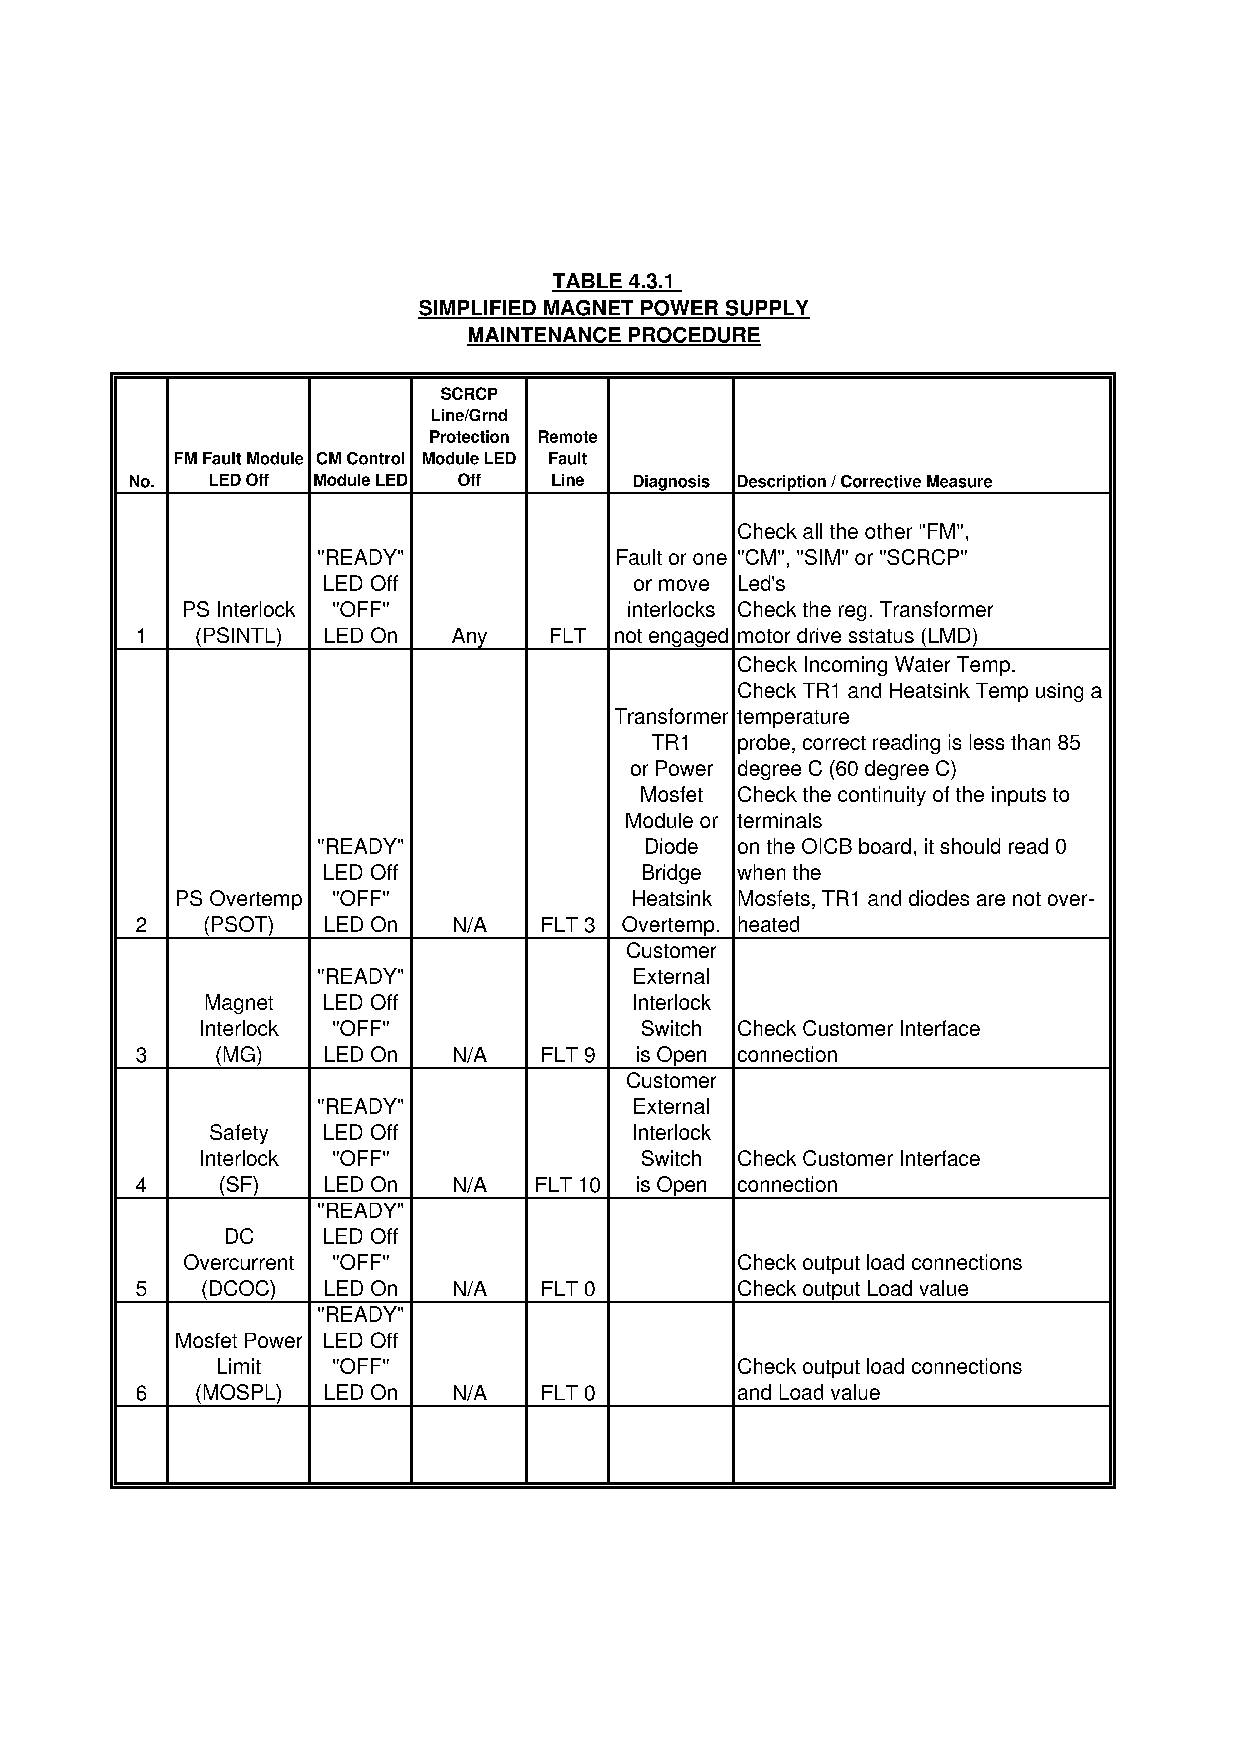
\includegraphics[height=7.5in,width=6.2in]{book1}
\end{table}

\clearpage
\begin{table}
\caption{Power Supply Maintenance Procedures (2 of 5) \label{tab:ps_maint_2}}
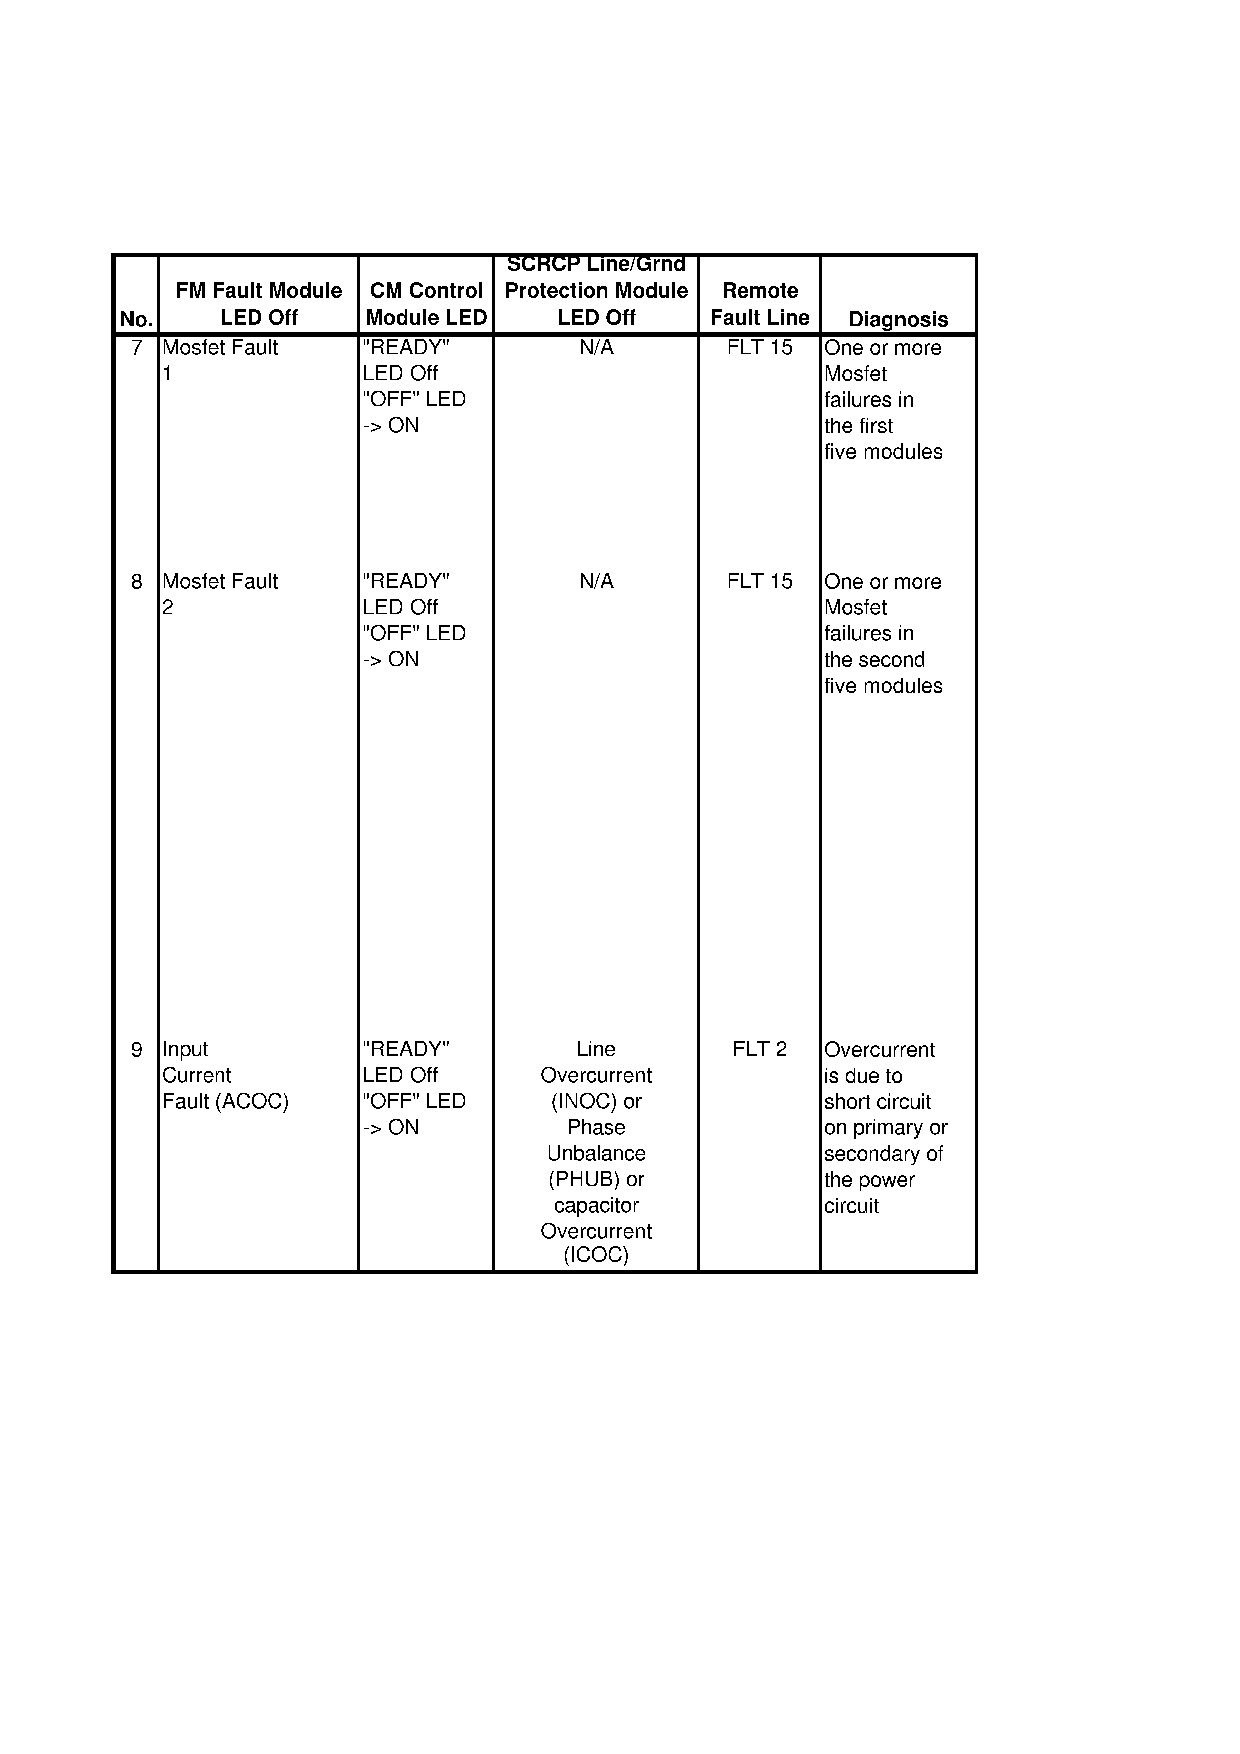
\includegraphics[height=7.5in,width=6.2in]{book2}
\end{table}

\clearpage
\begin{table}
\caption{Power Supply Maintenance Procedures (3 of 5) \label{tab:ps_maint_3}}
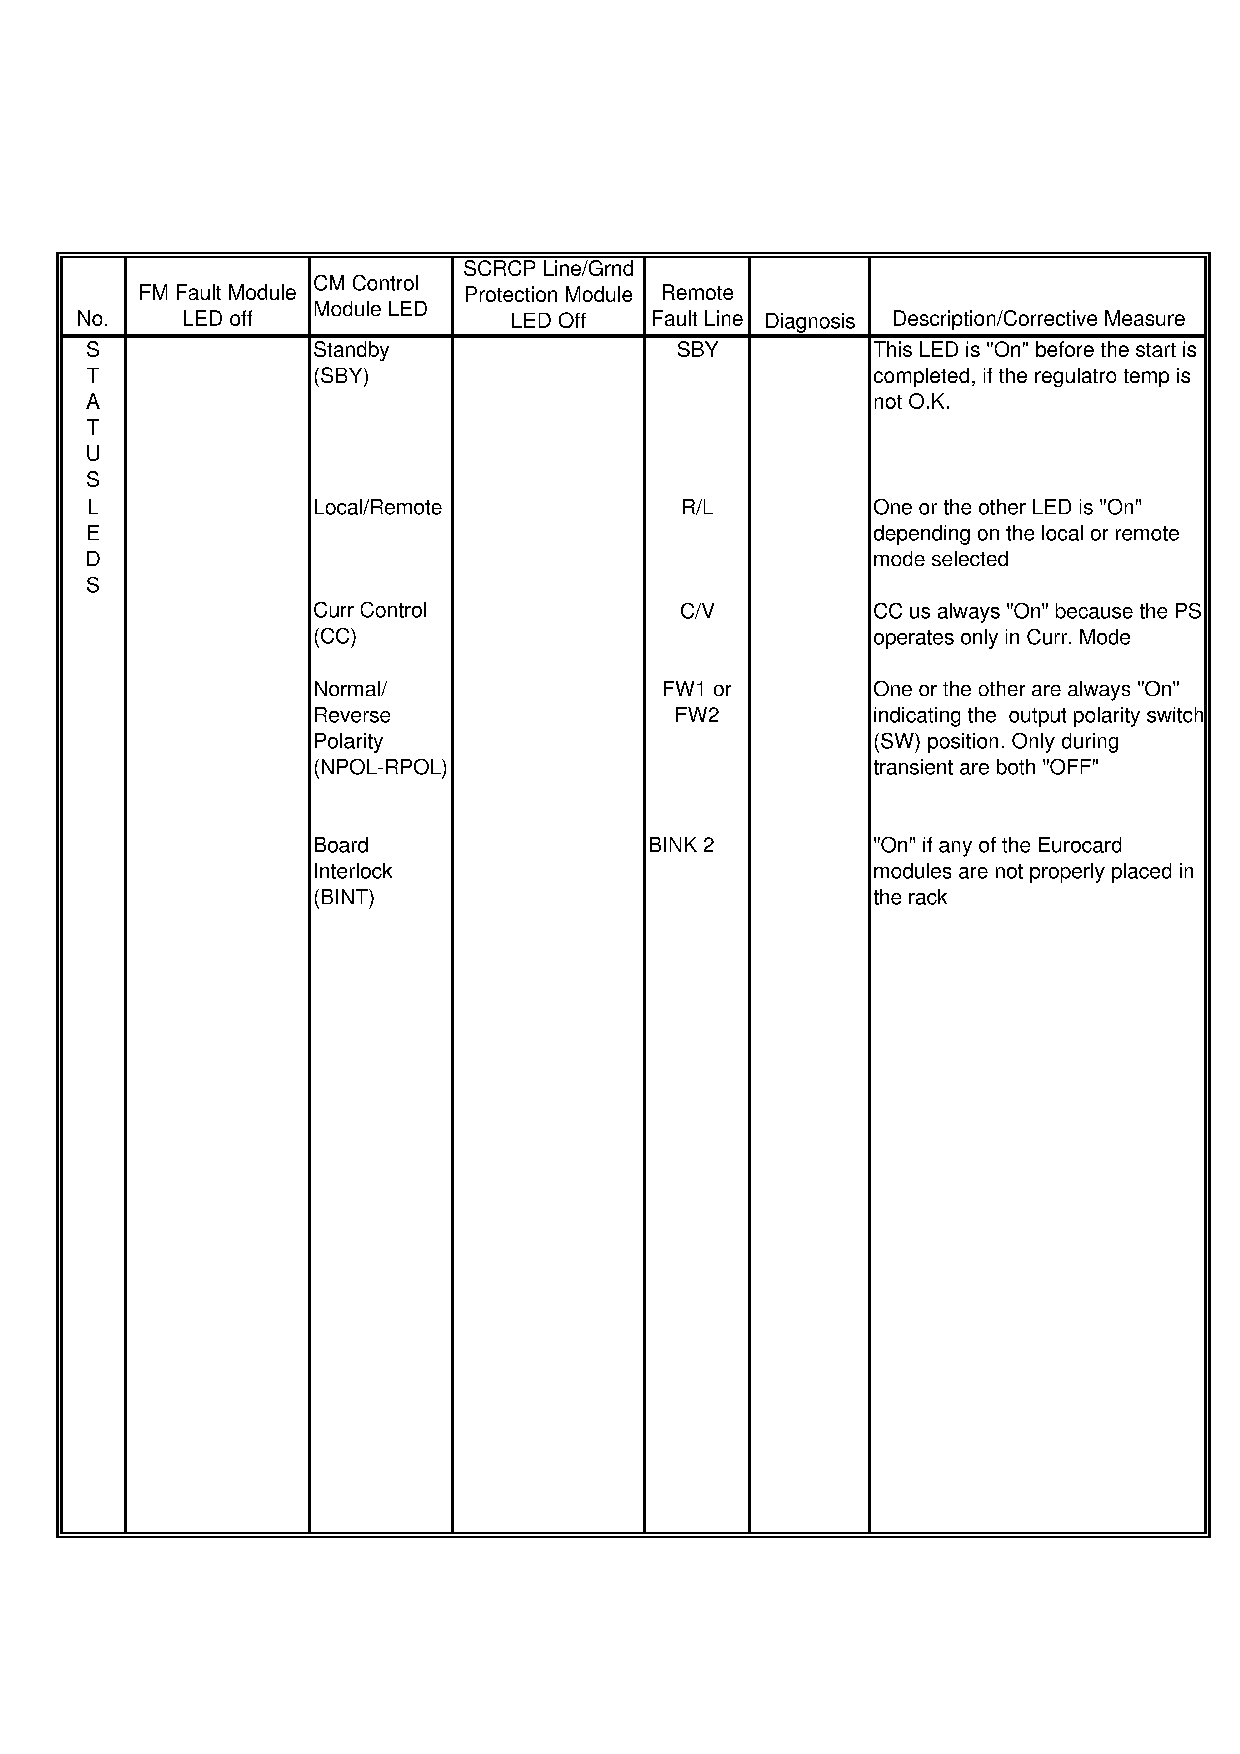
\includegraphics[height=7.5in,width=6.2in]{book3}
\end{table}

\clearpage
\begin{table}
\caption{Power Supply Maintenance Procedures (4 of 5)} \label{tab:ps_maint_4}
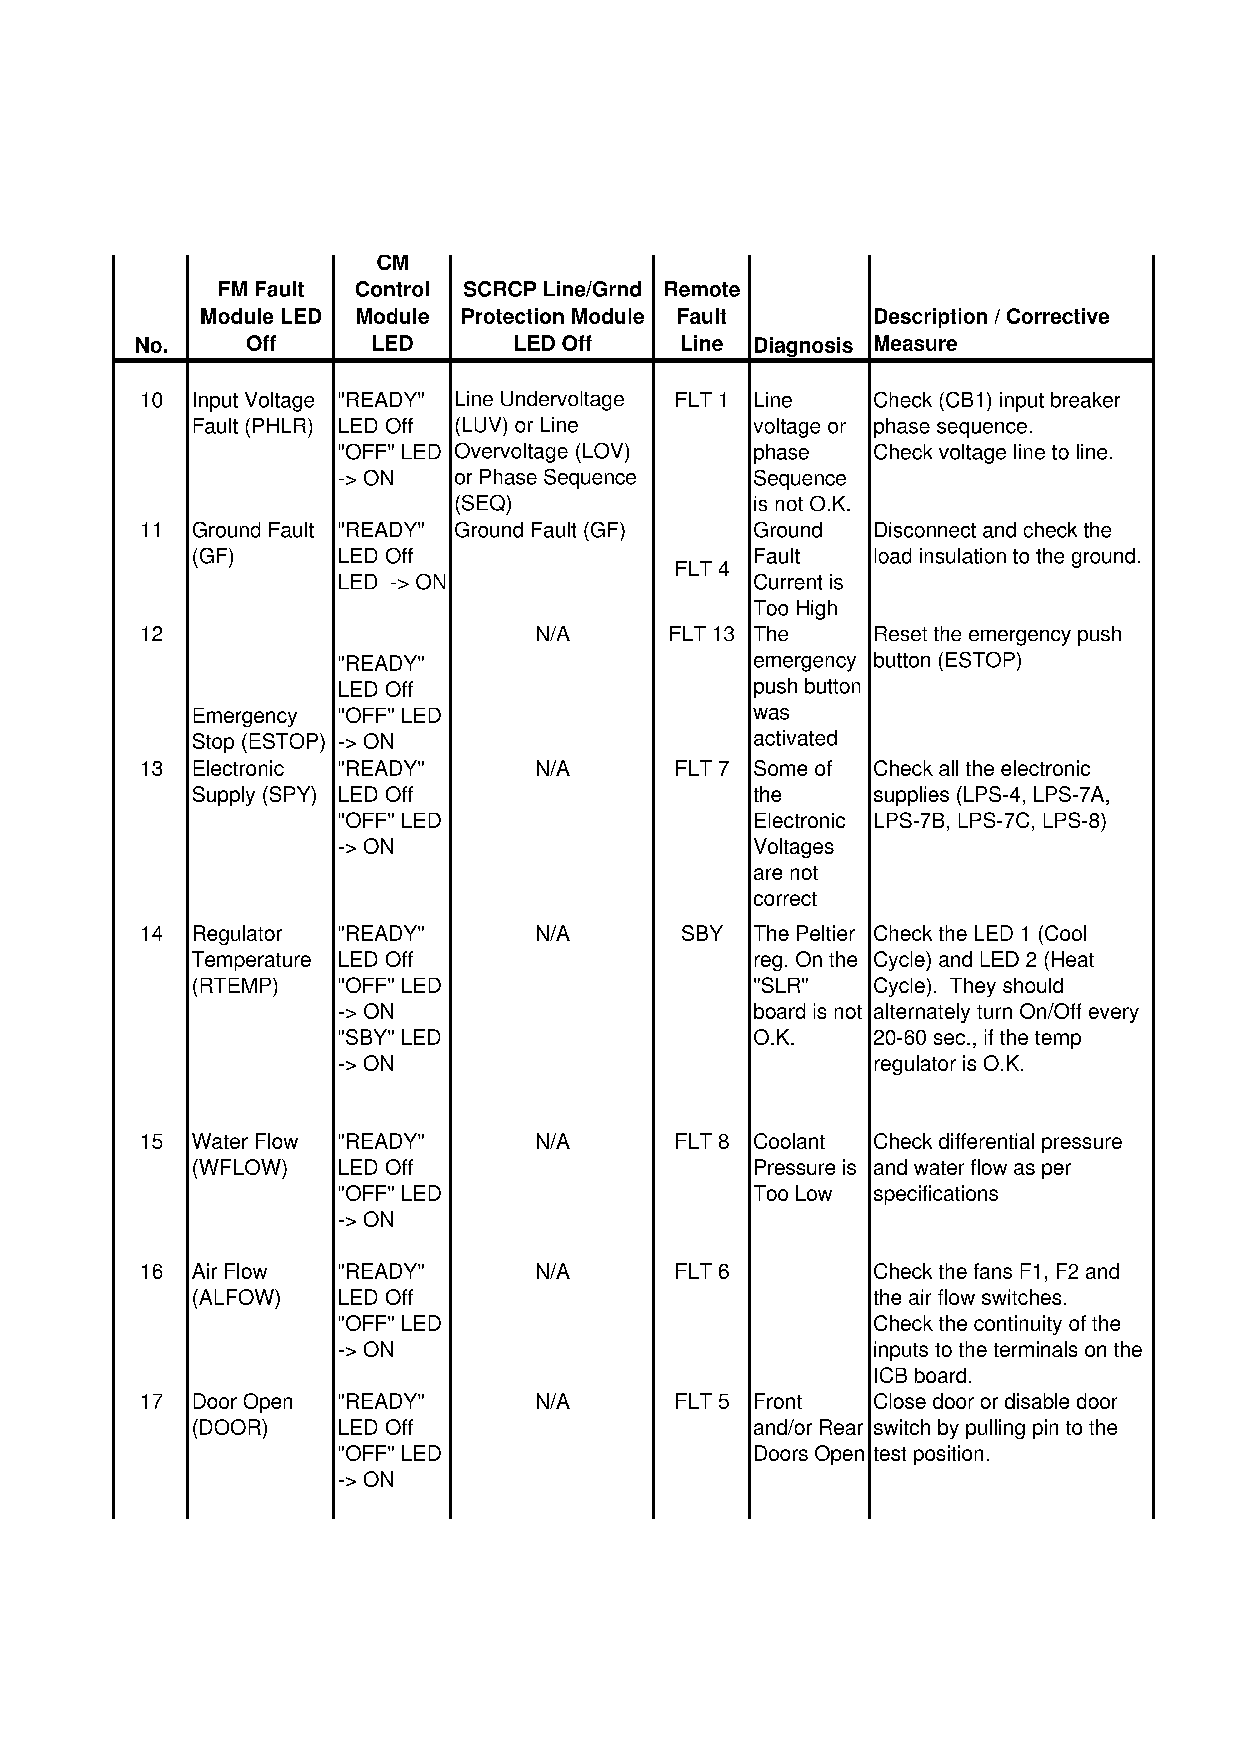
\includegraphics[height=7.5in,width=6.2in]{book4}
\end{table}

\clearpage
\begin{table}
\caption{Power Supply Maintenance Procedures (5 of 5) \label{tab:ps_maint_5}}
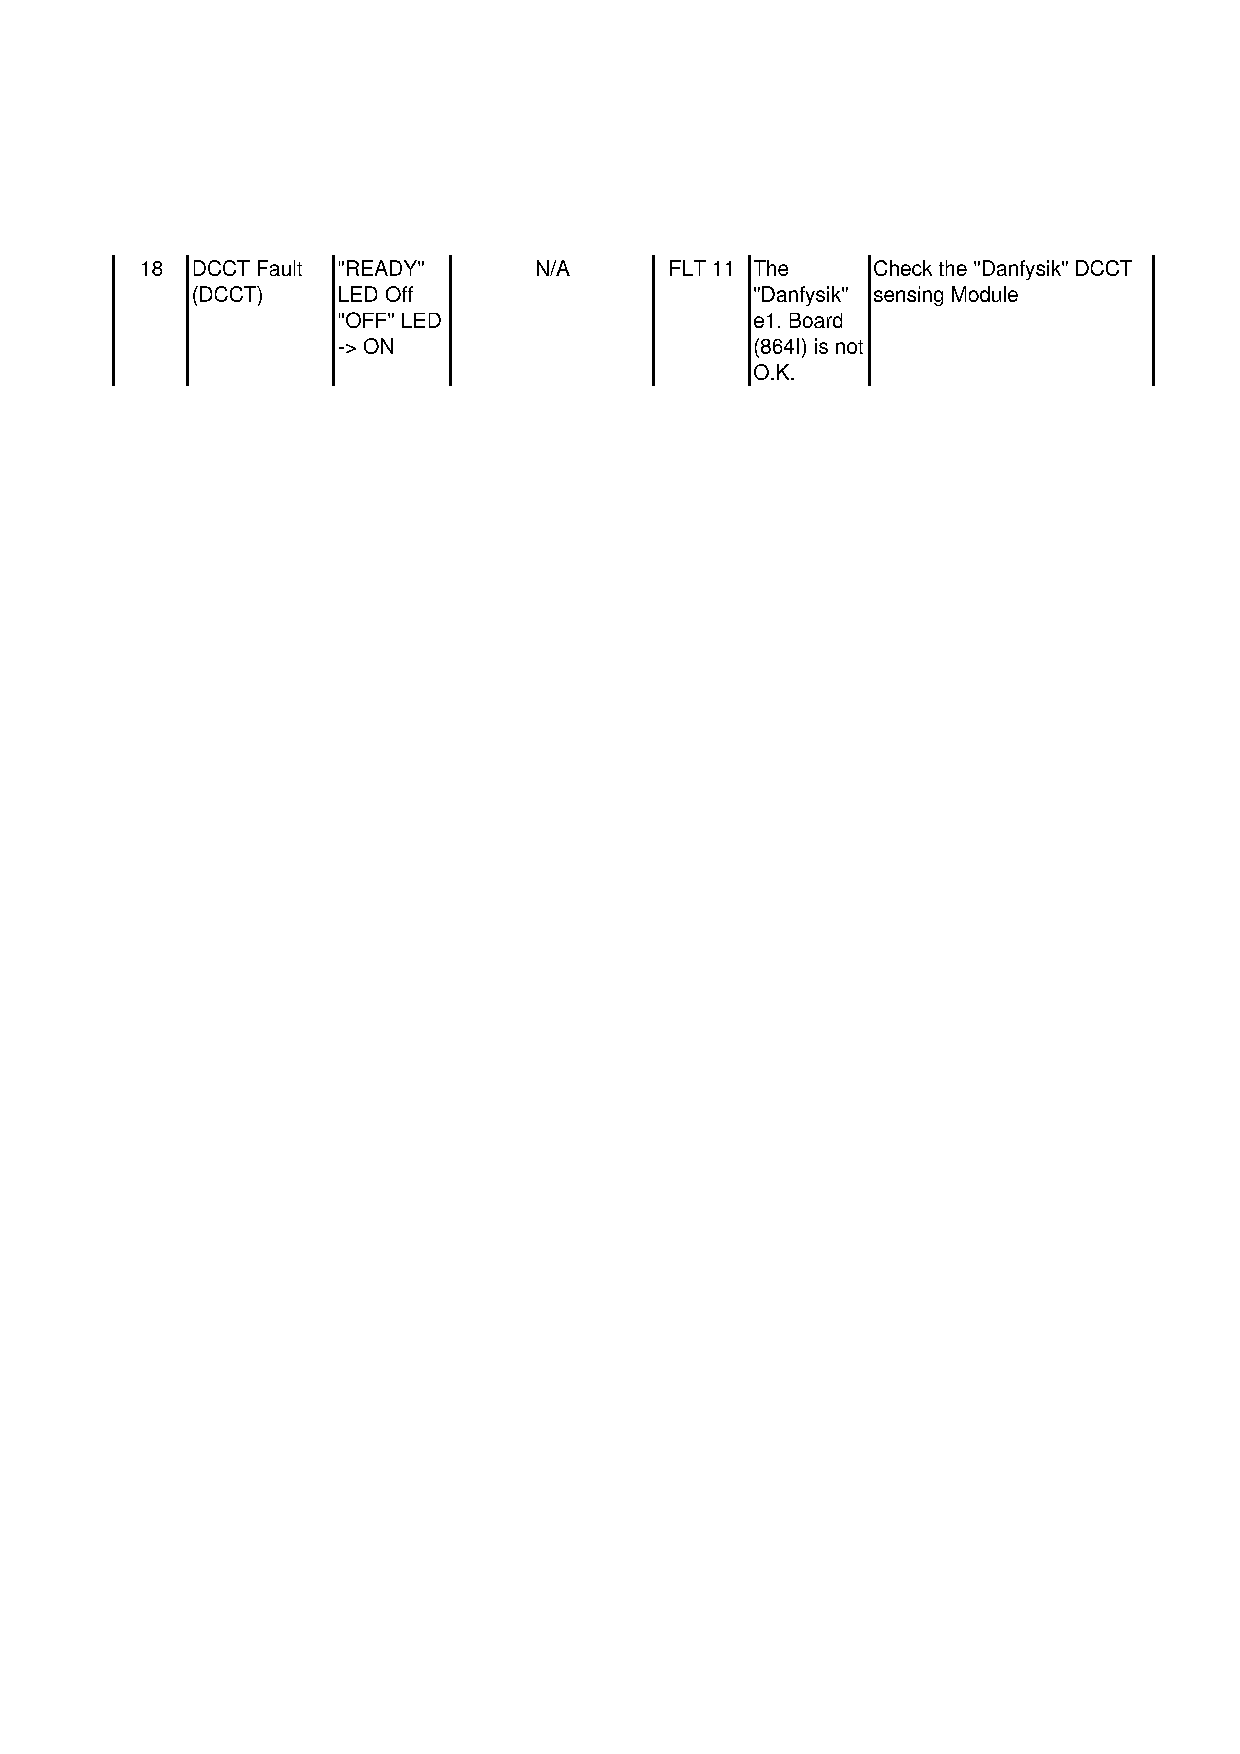
\includegraphics[width=6.2in]{book5}
\end{table}
\clearpage


\subparagraph{Device Changing Procedure}

When changing a puck device, the clamp nuts must be removed by
quarter turns of the wrench alternating between nuts.  See device
changing procedure below:

\begin{enumerate}
\item Remove gating leads from defective device (if applicable).
\item Loosen clamp torque-nuts by alternatively loosening each nut
1/4 turn.
\item Pry apart the bus bar, holding the device in place.
\item Replace the SCR.  Coat the SCR surfaces with Alcoa EJC joint
compound. Note the device polarity and orientation.
\item Tighten the torque nuts finger tight, ensuring that each has
been tightened evenly, and that the torque spring bar is perpendicular
to the SCR stack.
\item Tighten the torque nuts with a torque wrench by alternately
tightening each nut 1/4 turn until 160 inch pounds has been applied on
each.
\item Reconnect all gate leads and power leads.
\end{enumerate}

When changing a MOSET on a power module, the control wires and
water connections must be removed (quick connects).  The module can be
pulled out by pulling on the module handle.  Before mounting a new
device, a thin coat of Alcoa EJC joint compound should be applied to the
MOSET surface.  MOSETs are tightened to the heat sink only by two
screws.  After replacement, one has to make sure that all the wires are
returned to the right connection points.


\paragraph{Special Tooling}

The following power electronics instrumentation is required to
service the PS unit:

\begin{enumerate}
\item Dual Beam Oscilloscope c/w 10 x probe.
\item Good quality Multimeters.
\item Diode/SCR Tester.
\item 500/1000 volt dc/ac Megger.
\item 1000 volt ac/dc Voltmeter.
\item 300 in/lb capacity Torque Wrench.
\end{enumerate}

It is beneficial to have a lifting tool or equipment capable of
2500 lbs (1140 kg) for removal of magnetics (TR1, TR2, LF). These
components are front and rear exited from the enclosure.


\paragraph{Safety and Preventative Maintenance}

\subparagraph{Safety}

The Maintenance Technician should become familiar with the layout
and be aware of basic system parameters.  Only qualified technicians
should be allowed to work with this equipment under competent
supervision.

The DC Bus Capacitor in the power conversion compartment could be
charged up to 290 VDC volts.  These will normally quick discharge in
``Off" mode through CDR contactor and RD resistors.  The time to
discharge is approximately one (1) second.  In any case, check the DC
bus voltage, before servicing the unit.

The Technician must be aware of the energy sources fed into the
PS unit.  This is 480V, 60 Hz, 3$\phi$.  The 120 Vac for the auxiliary
circuits and electronics is derived from that voltage through F4, F5
fuses and TR3 transformer in the rear compartment.

\subparagraph{Preventative Maintenance}

General housekeeping is the key to maintaining power electronic
and electrical equipment.  The area is to be kept clean and as dust free
as possible when doors are open.  A schedule program of inspection will
reduce the possibility of problems.

After the first month of operation it is recommended that all
hose clamps, power connections and circuit board connections be checked.
 The procedure should be repeated after six months and every year
thereafter.

\begin{description}
\item{1.} Power Components - Electronic
\item{}\hskip0.3in To be kept clean and free of dirt and obstructions.
This will avoid tracking and heat build-up, thereby increasing the life of the
devices.
\item{2.} Capacitors
\item{}\hskip0.3in Capacitor forming takes place each time the PS is started.
If the PS has not been started in six (6) months, the CF electrolytic
capacitors may require reforming.
\item{3.} Control Components - Electronic
\item{}\hskip0.3in The Printed Circuit Boards are to be kept clean and free
of any accumulations of dirt and foreign material.
\item{}\hskip0.3in Static materials should never be allowed near PCB's while
in PS or in stores.  Caution should be used when near or handling PCB's.
\item{}\hskip0.3in There are no special requirements (other than housekeeping
standards) for the maintenance of the logic control components.
\item{4.} Power Components - Magnetic
\item{}\hskip0.3in General housekeeping and clean environment.
\item{Note:} All Items above are subject to thermal degradation and good
housekeeping is the prime method of maintaining original design
parameters.
\item{5.} Plumbing Components
\item{}\hskip0.3in The major components requiring preventative maintenance are
in the plumbing system.
\item{}\hskip0.3in Periodic checking of the water pressure annunciations will
ensure that water flow reduction will give the appropriate alarm.
\item{}\hskip0.3in Turn the unit's cooling circulation ``ON".  Check all hose
connections for leaks or looseness.  Check for any worn hoses (at
clamps) due to heat.
\end{description}
\end{comment}

\begin{comment}
\section{SOS Vacuum System }

The entire volume of the SOS spectrometer, from the entrance window in the
front of the quadrupole to the exit window at the exit of the second dipole,
inside the detector hut,
can be evacuated. This in order to minimize the effects of multiple
scattering on the SOS performance. As is the case with HMS vacuum can,
the entrance and exit are covered
by mylar-kevlar composite vacuum windows.

The spectrometer vacuum is maintained by a single Leybold 1000 liter
turbo pump and the vacuum is read with a cold cathode gauge.
This can be displayed on one of the TV monitors in the Hall~C
counting house.

Since the exit window of the SOS vacuum system has under 1/3 the stress of the
large HMS exit window, and has a very sizable safety margin,
no kevlar ``Blast Shield" has been installed.
Signs indicating the presence of thin vacuum windows have been posted in the
shield house and at the pivot point.


\section{SOS Slit Systems}

\subsection{SOS Slit Box}

The SOS slit system is directly mounted to the vacuum can of the SOS quad.
Like the HMS slit system, it consists of a vacuum box with a slit
ladder mounted into it. The slit ladder has space for three separate slits,
which will typically be one sieve slit and two solid angle defining collimators.
The slits are rectangular blocks of densimet (90\% W and 10\% Cu/Ni)
with a density of 17 g/cm$^3$. The collimators have an octagonal shaped
opening machined into them, the sieve slit has many holes drilled
into it.

The outer size of all slits (solid-angle defining collimators and
sieve slits) are 8.25" vertical times 11.75" horizontal.
The central hole of the sieve slit has a smaller aperture, and two blocked
holes exist to easily distinguish center and directions. Next to this
the horizontal spacing of the three innermost columns of holes is
reduced such that we can use the same slit when we run the SOS spectrometer
in its parallel-to-point tune (default is point-to-point).
The collimator thicknesses are 2.5", while the sieve slit thickness
is 1.25". The dimensions and shape of the inner aperture of the present
SOS collimators is included in Table~\ref{tab:apertures} in the section on the HMS 
 slit system.

Similar to the HMS aperture,
the total depth of the slit box is close to 3.75", which leaves
enough space to later mount scintillators behind the collimators as an active
veto counter (to prevent punch-through of hadrons) and/or to increase
the collimator thickness. Two circular quick-connect flanges are
added for feed-through of possible light guides.

The remote control system for the SOS slit system is completely analogous
to the HMS slit system (see Section~\ref{sssec:slit_control}),
and built into the same control box
(behind the blue power supply racks on the floor of Hall~C).
Four buttons are included on the front face for SOS, denoting ``home" and
the three slit positions.
The emergency button shuts down the full control system, and thus both motion
of HMS slit ladder and SOS slit ladder.
\end{comment}
%\subsubsection{Movable Jaw System}

%To the front of the SOS slit box a 10" inner diameter gate valve is installed.
%In front of that one either installs a 11.1" long vacuum spool piece,
%for normal operations, or the so-called ``SOS Movable Jaw System."
%The latter system is borrowed from SLAC and consists of an independent
%horizontal and vertical movable slit system, to be used for calibration
%purposes. {\bf Note that with this system installed the minimal scattering
%angle SOS can obtain is limited to 21 degrees.}
%All slits or jaws consist of Tungsten with a layer of Copper around it.
%The vertical moving
%slits have a (rectangular) size of 4.5" high times 10" wide times 4" thick,
%and can move independently. The horizontal moving slits have a
%(rectangular) size of 12" high times 5.5" wide times 4" thick, and are
%moved together by a single motor.
%Motion of the jaws is performed by applying 110 V through a push-button-relay
%system to three single-phase AC motors, while visual displays show the optical
%encoder settings. To move control from down in Hall~C to up in the counting
%house, and vice-versa, one has to swap cables.

\begin{comment}
\subsection{Hazard Identification}

The principal hazards are
\paragraph{Magnetic} There is a significant fringe field at
the entrance and exits of the magnets. This represents a hazard
to workers handling magnetic objects (tools) and to personnel with
pacemakers. In addition the field could erase magnetic
information storage media such as the strips on credit cards.
\paragraph{Mechanical}
In front of the SOS slit box a vacuum gate valve is mounted.
In its normal operation mode a metal gate will be closed with
severe pressure when the electrical power drops. This can cause serious
damage to interfering body parts.
A similar problem involves the slit ladder itself. The total weight of
the three slits amounts to approximately 350 Lbs (160 Kg) and can easily
cause serious damage to body parts.

\subsection{Hazard Mitigation}

\paragraph{Magnetic} A sign will be posted which indicates the presence of 
a high magnetic
field ( this is standard JLab safety signage). The exact wording is
`` High Magnetic Field - No Pacemakers or Credit Cards." There are also
flashing red lights located on the HMS carriage indicating that the
magnet power supplies are energized. Be careful with tools (magnetic?)
when you work on the slit boxes with the red lights in a flashing state.

\paragraph{Mechanical} When performing manual labor in the vicinity 
of the vacuum gate
valve either close the gate valve or block the gate valve such that
it can not accidentally close on you.

When installing the slit ladder, be careful when you work with your hands
under the slit ladder (like when you are bolting the slit box to the
gate valve). Remove the slit ladder, or {\bf install a support under the slit
ladder to prevent it from falling all the way down}.

A brake system has been included in the control to prevent the slit ladder
from sliding down in case of a power failure.

The SOS movable jaw system {\bf only} moves when power is available and
a push-button is used. Its default is not to move at all.

\section{SOS Carriage and Rotation System }

\subsection{Introduction}

	The Carriage is the support structure of the spectrometer.
Note that the safety issues associated with the carriage are not included
in the \htmladdnormallink{ESAD}{http://www.jlab.org/Hall-C/document},
and will be discussed here.

First and foremost as it is a multi leveled structure, it is important to keep in
mind that people may be working above you. This means that hard hats should
be worn.

The steps to enter the SOS carriage are at the back of the spectrometer.
The first level of steps brings one to the electronics shed, where all
SOS data acquisition electronics and cable racks are located.
A second level of steps brings one to the platform along the
shield house, giving access to all detectors and the SOS High Voltage
power supplies.
A third level of steps leads
to the top of the spectrometer, where the motor to control the door
mechanism and the hut air conditioning system are situated.
Access to this level should be limited to
persons performing maintenance or repair work. A chain normally
prevents access to this level.

On all stages of the SOS carriage
all the usual precautions associated with heights should be followed.
Safety railings have been installed everywhere along the carriage perimeters.

The entire spectrometer can be rotated. The angle of the spectrometer
can be manually determined using a plumb bob attached to a reference mark on the
carriage frame at the rear of the spectrometer.
This plumb bob is aligned over survey marks which have been painted
on the floor in red at 0.5 degree intervals. Rotation of the spectrometer
is accomplished by using the two motors on the carriage itself.
These AC motors are controlled by synchronous pulse width modulated
drives which are mounted near the bottom of the shield house steps.

\paragraph{Remote Rotation}


During rotation constant visual inspection with the two wide-lens, zoom Hall~C
cameras is obligatory. This visual inspection should ensure that nothing
blocks the spectrometer path (either on the rails or on the floor), that there
is no interference with either HMS or beam line, and that the flexible cable
trays do not get stuck.

Limit switches will be installed at forward
and backward angles which prevent SOS to rotate to angles more forward than
20 degrees. To obtain more forward or more
backward angles an access is needed, and rotation has to occur manually
downstairs with spotters. Hard limit switches will be installed to prevent
the spectrometer to rotate out of their maximum allowed range.

In case the SOS spectrometer is rotated to more forward angles, pay especially
close attention to interferences between the HMS and SOS. Up to this moment the closest angle
distance we have obtained between SOS and HMS is 35 degrees.

Remote rotation  is accomplished via the PLC remote controller in the Counting House. 
Remote spectrometer rotation occurs by computer. Commands can be
issued to a PLC (Texas Instruments 5000), which executes these commands
following algorithms stored in its memory. The PLC is situated at the first
level of the HMS carriage, opposite to the magnet power supplies.
The advantages of using the PLC are:

\begin{itemize}
\item{No direct access by users to the algorithms, preventing unsafe
rotation attempts (instead, the algorithms have to be loaded locally into
the PLC).}
\item{Rotation of both HMS and SOS by the same smart controller, enabling
security checks of both angle decoders. This renders a better handle on the
minimum allowed angle in between both spectrometers.}
\item{Automatic slower rotation speeds (if desired) if close to desired angle
when using proximity switches.}
\end{itemize}

The PLC communicates directly with the control electronics of several limit
switches, proximity switches, and decoders. Next to the limit switches
also hard limit switches will be installed on the floor, to prevent failure
of the PLC limit switches.


\paragraph{Manual Local Rotation by Authorized Personnel}

The spectrometer motors may only be controlled by trained personnel.
Manual remote rotation of the SOS may only be done by the 
Hall~C staff members responsible for the Carriage and Rotation
System (listed in the 
\htmladdnormallinkfoot{ESAD}{http://www.jlab.org/Hall-C/document}).  
At least two people are required for spectrometer rotation, one to
run the motors and at least one spotter. Prior to rotating the spectrometer
a visual inspection of the area should be made to insure that there
is nothing in the path of the spectrometers or on the rails. During rotation
the spotter should pay special attention to the flexible cable ducts,
to make sure that nothing is hung up or stretching.


\subsection{Carriage}

The Short Orbit Spectrometer steel carriage consists of four pieces; a pivot
section; main carriage body and two pairs of locomotive style wheels. On
top of the carriage is a concrete detector shield house. Attached to the rear
of the concrete shield house is a prefab steel electronics hut. Personnel
access is provided to the electronics hut, shield house door (and to the
target area near the pivot).

The concrete shield house is constructed of high density concrete with
0.5\% boron frit (by weight) additive. High density concrete contains
aggregate that is 66\% iron ore and is almost 40\% heavier (208 lb/ft$^3$) by
weight than standard concrete (150lb/ft$^3$). The concrete is 24" thick on all
six sides. The inside walls and roof of the shield house are lined with panels
consisting 2" of lead poured into boxes with 1/4" steel sides. The rear
interior wall and the shield house floor are lined with 2" steel plates.

Access to the detector stack is through a vertically opening counter
weighted door. The door operates by electronically controlled hydraulic
cylinders.

\subsection{Pivot}

The SOS pivot surrounds the top half of the center pivot in Hall~C. The
pivot section is bolted to the main carriage. The SOS has two bearing
surfaces upon which it moves. The cross roller bearing provides horizontal
rotation. The spherical bearing allows out of plane movement.

Both bearing surfaces are lubricated with grease. Periodic regreasing of
these bearings will eliminate problems.

The spherical bearing race is provided with grease zircs that are accessible
through access cut-outs in the pivot housing. The bearing should be
regreased before out of place movement if out of plane operation is infrequent.
Two surfaces of the spherical bearing race are covered with Teflon
film. When the Teflon deteriorates the bearing will need to be greased more
often. Failure to grease the bearings could result in rough movement and
binding. The cross-roller bearing has several grease zircs along the top
surface of the spherical bearing race.

\subsection{Wheels and Angle Readout}

The SOS wheels are constrained to rotate on a track 35' from the central
pivot. Each wheel pair contains a drive wheel and an idler wheel. Each
drive wheel has its own motor and controller. The design allows the
spectrometer to rotate with just one of the two motors operating. The
recommended procedure is for running two motors together as this reduces stress
on the system. The motor controllers are located in a steel cabinet at the
bottom of the stairway at the rear of the spectrometer. The controllers are
supplied with 480V. The circuit for these is in the C-UPH3 box on the non-door
side of the shield house. There is not an ``ON" switch, the controller LED's
are lit if the circuit is on. Past experience has shown that 30Hz setting is a
reasonable movement rate. This results in a change of approximately 1
degree per minute. Fine adjustment can be made at 10Hz pretty easily.

{\bf The forward direction on the controller is a counter-clockwise rotation.}

There is a white C-beam welded to the centerline of the carriage a few feet
downstream of the track. A scribe line on a red background at its base is
used for angle positioning by aligning to survey marks on the floor. The
scribe line is along the same centerline used to align the dipole and quadrupole
magnets. A camera is mounted to the beam to allow
remote visual readout. Manual control involves starting and stopping the
motor(s) by hand until the desired angle is reached.

\subsection{Rotation}

\paragraph{Pre-Rotation Checkout}

Prior to rotation the track should be inspected and cleared of objects. This
includes the track area under the carriage between the wheels. Previously,
the track has had brooms, nuts, bolts, water hose and cables lying across it.
All obstructions must be moved before the SOS is rotated.
The area around the spectrometer also needs to be cleared of materials.

If the track is clear, rotation between 20 degrees and 140 degrees is not a
problem. At angles smaller than 20 and larger than 140 degrees care must
be used to prevent the SOS from hitting stuff. The data cable ``elephant
trunk" under the SOS needs to be monitored and moved so that it does not
bind and tear loose from its' mounting points. The fouls at small angles are
related to the scattering chamber, beam dump vacuum pipe, the HMS and
the cables and connections on the SOS quadrupole. At large angles the
SOS will foul with the beamline and the access stairway near the pivot.
Rotation at a slow speed with persons watching from the pivot area can
avoid equipment damage. Until the quadrupole is refitted with a new coil
the minimum angle possible is 18 degrees.

\paragraph{Manual Rotation}

To rotate the SOS manually perform the following steps:

\begin{enumerate}
\item{Inspect and clear the track.}
\item{Turn on the motor circuits 8,10,12 and 14,16,18 in circuit box C-UPH3}
\item{Secure the door to motor the controller box open}
\item{Set frequency as desired (30Hz for general movement 10Hz for fine
control)}
\item{Press forward or reverse direction to move spectrometer.}
\item{Press stop at the desired angle.}
\item{Repeat if desired.}
\end{enumerate}




\subsection{Out-of-Plane Jacks}

The Short Orbit Spectrometer is designed to allow out-of-plane operation.
Two hydraulic jacks are attached to the rear section of the carriage. They
can be used for leveling the spectrometer and lifting the SOS out of plane. A
third large hydraulic cylinder is attached diagonally from the right jack
base to the bottom of the carriage on the left.  Presently use of
this system is disabled.

The design allows a 20 degree tilt above the beamline. When the SOS
wheels are on the rails the spectrometer is declined by 0.15 degrees below
the beamline. Until a jack control system is available to level the
spectrometer the SOS will be declined during data taking.
\end{comment}

